\documentclass[12pt,a4paper]{article}

\setlength{\textwidth}{165mm}
\setlength{\textheight}{240mm}
\setlength{\parindent}{0mm} % S{\aa} meget rykkes ind efter afsnit
\setlength{\parskip}{\parsep}
\setlength{\headheight}{0mm}
\setlength{\headsep}{0mm}
\setlength{\hoffset}{-2.5mm}
\setlength{\voffset}{0mm}
\setlength{\footskip}{15mm}
\setlength{\oddsidemargin}{0mm}
\setlength{\topmargin}{0mm}
\setlength{\evensidemargin}{0mm}


\usepackage[T1]{fontenc}
\usepackage[all]{xy}
\usepackage{graphicx}    % For grafik (billederfiler)
\usepackage[T1]{fontenc} % For at blande \textsc{} med \textbf{}
\usepackage[utf8]{inputenc}
\usepackage{amsfonts,amsmath,amssymb}
\usepackage{eucal}
\usepackage[danish]{babel}
\usepackage{enumerate}  
\usepackage{hyperref}
\usepackage{url}
\usepackage{array}
\usepackage{mathptmx}
\usepackage{amsmath}
\usepackage{multirow}
\usepackage[dvipsnames,usenames]{color}
\usepackage{tabularx,colortbl,xcolor}

\DeclareSymbolFont{usualmathcal}{OMS}{cmsy}{m}{n}
\DeclareSymbolFontAlphabet{\mathcal}{usualmathcal}



\begin{document}
\title{PKSU Delrapport 2}
\maketitle
\begin{center}
Jeppe Schönemann Skov, Rose Sofie Greve, Frederik Leed Henriksen \\ \hfill \\ \hfill \\ 
\end{center}
\newpage
\tableofcontents
\newpage
\section{Abstract}
We are making a website for a small Bed and Breakfast on Isla Margarita, Venezuela. The place is working towards becoming a sustainable and self-suffficient mini-hostel, where guests can enjoy organic greens from the garden.
The indexpage on the website will contain a description of the place and the surrounding area.
The website will contain a simple booking- and online payment system.
The website will have a link with pictures of the houses and surrounding facilities, and a link with information on the different activities taking place at the hostel.
With courtesy to the place working with ecology and sustainability, the layout of the website will be simple and inspired by the colors of nature.
Further, we will make an administrating part of the system, from where our costumer can see and edit the bookings. The administrator will also be able to edit the website photos and text descriptions. 
\newpage
\section{IT-projektets formål og rammer}
F. Skal indeholde et bookingsystem og information om hostel \\

A. Skal administrere bookninger, herunder til- og afmelde folk samt finde kontaktoplysninger på de folk der har oprettet en booking.\\
 
C. Udvikling og endeligt brug af systemet skal være minded på, at dem der skal betjene det, ikke har stor teknisk erfaring. Vi skal derfor udvikle minded på, at de tekniske detaljer ikke er deres fokus.\\

T. Systemet skal både udvikles og kunne betjenes på en billig pc med internet. Ingen yderligere krav er på nuværende tidspunkt planlagt. \\

O. Mennesker der søger at booke værelse. Organisering af hvilke værelser der er ledige og hvor længe.\\

R. Systemet skal løse administrative problematikker i henhold til at holde styr på kontaktoplysninger af kunder. Holde styr på hvilke værelser der er ledige, og hvornår disse er ledige. Systemet skal også reklamere for hostel'et.\\
\newpage
\section{Kravspecifikationer for IT-løsningen}
\subsection{a}
\textbf{Funktionelle krav:} \\
	Systemet skal understøtte et bookingsystem, der indeholder kontaktoplysninger om kunder, 	samt muliggører bookings af kunder, og at administratoren kan booke/af-booke kunder. Desuden skal der være et betalingssystem, så man kan betale online \footnote{Vi har ikke på nuværende tidspunkt tilstrækkelig indsigt i, hvorledes et betalingssystem skal kunne fungere, eller hvordan man man kan implementere dette, til at vi har ladet det være en del af resten af de tekniske kravspecifikationer, indtil vi har en dybere forståelse af dette. Det er altså et projekt, vi tager fat på senere i udviklingen (men det er ikke glemt!)  } \\ \hfill \\
       \textbf{Ikke-funktionelle krav:} \\
	Systemet skal være brugervenligt i henhold til folk uden megen teknisk erfaring. 	Hjemmesiden skal indeholde billeder/information om hostelet. Siden skal være i farver og 	stil der afspejler hostelets stil og holdning til miljøet. \\ \hfill \\
      \textbf{Begrænsninger:} \\
	Siden skal kunne vises på en billig computer og uden hurtigt internet til rådighed.
\subsection{b}
Der er vedlagt et billede, der illustrerer, hvorledes administratoren skal logge ind. Men derved også har ret til at slette bookninger og hente information, om dem der bookede et værelse. Kunden skal ikke logge ind, men har så også kun ret til at booke.\\ 
\begin{figure}[H]
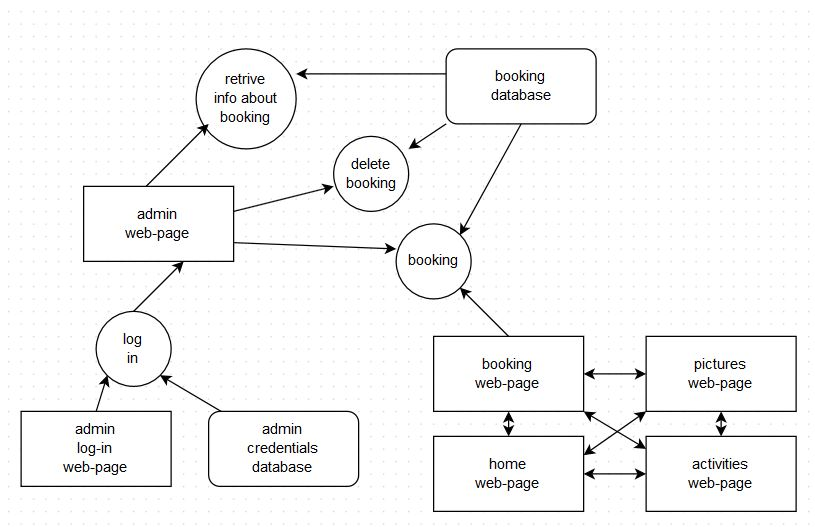
\includegraphics[scale=0.7]{useCaseModel.jpg}
\caption{Use Case model}
\end{figure}
\subsection{c}
\textbf{1.} Admin log-in. Her indtastes administratorens oplysninger på log-in skærmen. Dette bliver 	videreført til sikkerhedsverificering, som beder beholdningen af administrator oplysninger 	om at lede efter et match. Hvis dette match findes, bliver man logget in, ellers bliver man 	afvist. \\
	\textbf{2.} Admin interaktion. administratoren logger ind (trin 1), og kommer ind på 	administratorsiden. Her forespørger administrator siden om information på et rum eller at 	oprette/slette en bookning. Dette bliver sendt til validering, som tjekker om informationen er 	meningsfuld (fx om man vil oprette en bookning, til en dato der er passeret). Herefter bliver 	informationen sendt videre til booking databasen, hvor oplysninger bliver hentet og tilbage 	forbi validering, hvor man igen validere (fx om man opretter en booking på et allerede 	optaget værelse). Bliver forespørgselen på noget tidspunkt dømt invalid, vil man på 	administrator siden modtage passende fejlmeddelelse. Hvis alt går godt, vil man få sin 	information eller få at vide at oprettelsen/fjernelsen af en bookning skete planmæssigt.\\
	\textbf{3.} kunde booking. Her indtaster kunden sine oplysninger på booking siden, og disse 	oplysninger bliver sendt videre til validering (fx for få cifre i tlf. nummer). Passere kunden 	dette bliver forespørgslen sendt videre til booking databasen, som oplyser validering, om det 	ønskede værelse er ledigt for booking, hvorefter validering genevaluerer. Hvis forespørgslen 	er acceptabel, bliver ændringen gennemført, hvorefter kunden bliver informeret om en 		succesfuld booking. Hvis validation på noget tidspunkt i processen validerer til falskt, bliver 	processen stoppet, og kunden bliver i stedet mødt af en fejlmeddelelse.
\subsection{d}
Siden vi endnu mangler meget erfaring inden for web-programmering, er vi ikke sikre på, at følgende fremgangsmåde vil virke. Vores foreløbige ide til at lave et bookingsystem er som følger i billedet, at vi laver en klasse, som styrer de forskellige rum i hostelet(Main). Så laver vi en klasse, der holder styr på hvor mange senge, hvert værelse har samt en ”kalender” pr. værelse(Room). Så har vi en klasse, der holder styr på reservationerne(booking). Derudover er der en klasse, der holder styr på tidsenheder(), og en der holder styr på personinformation(Customer). Dette er indskrevet med java i tankerne, men vi er som sagt ikke klar over, hvordan man eksekvere kode i sin html-kode endnu, så dette er et work-in-progress.\\
\begin{figure}[H]
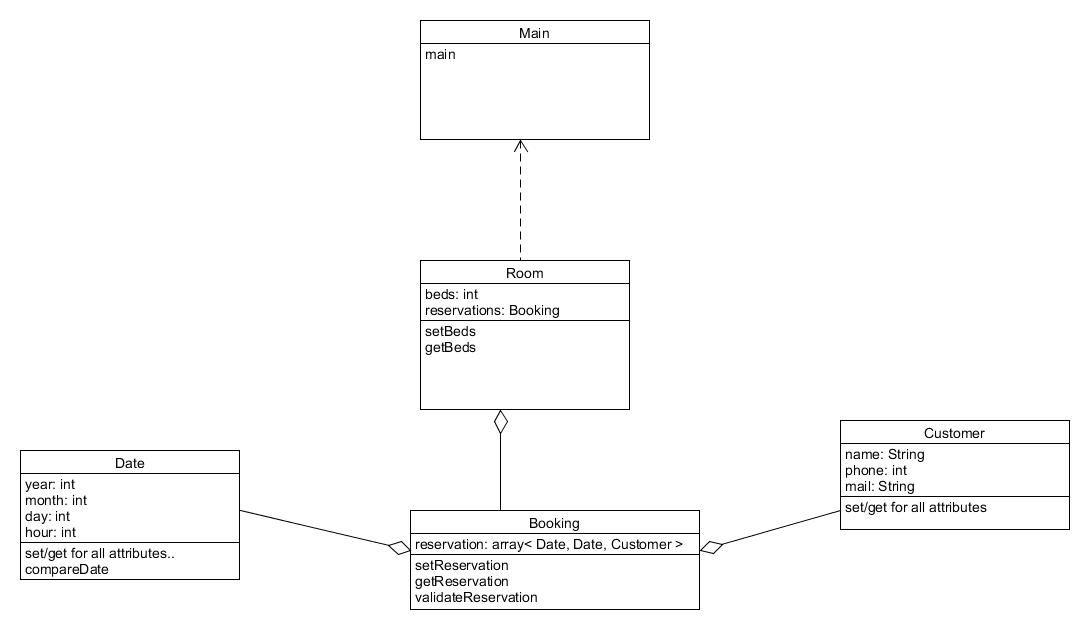
\includegraphics[scale=0.4]{unfinished.jpg}
\caption{Booking system - UML}
\end{figure}
\subsection{e}
”Home” siden og ”admin log-in” siden er vores  boundary objects, da de er det første i vores system, man støder på.
Vores entity objects omfatter alle vores web sider(udover dem der er boudary objects!), da de udgør en meningsfuld del af systemet. Derudover er vores ”admin credentials database” og vores ”booking database” også betragtet som entities, da de indeholder al information i systemet.
Vores control objects er ”admin log-in”, ”create booking”, ”delete booking” og ”retrive info”. Dette er de, fordi de ikke selv opbevarer noget information, men spiller en afgørende rolle i, hvad for noget infromation der bliver lagret/slettet. \\
\begin{figure}[H]
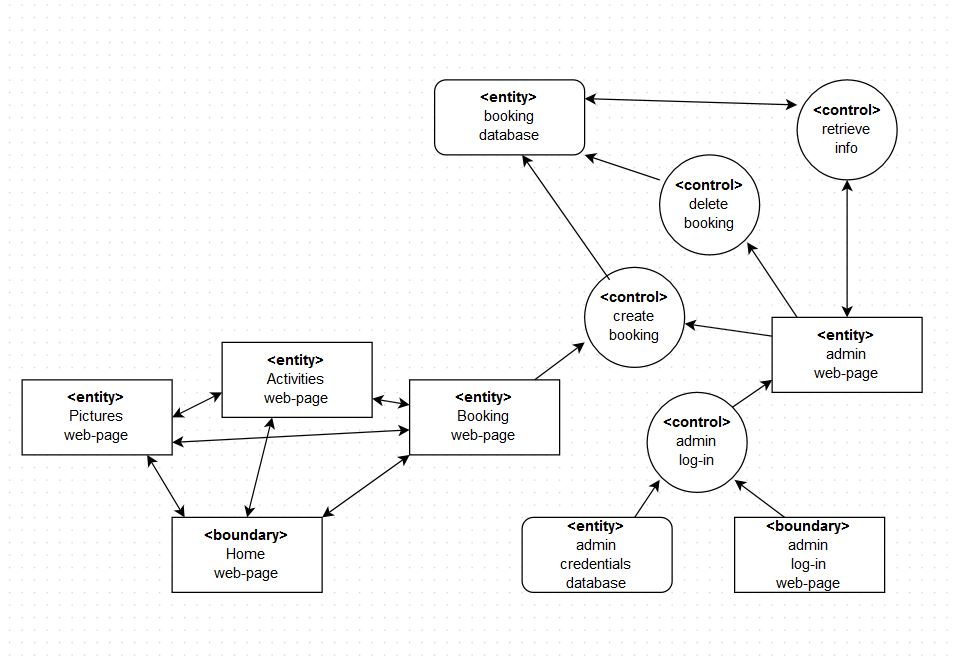
\includegraphics[scale=0.6]{BCE.jpg}
\caption{BCE Model}
\end{figure}

\subsection{f}

\begin{figure}[H]
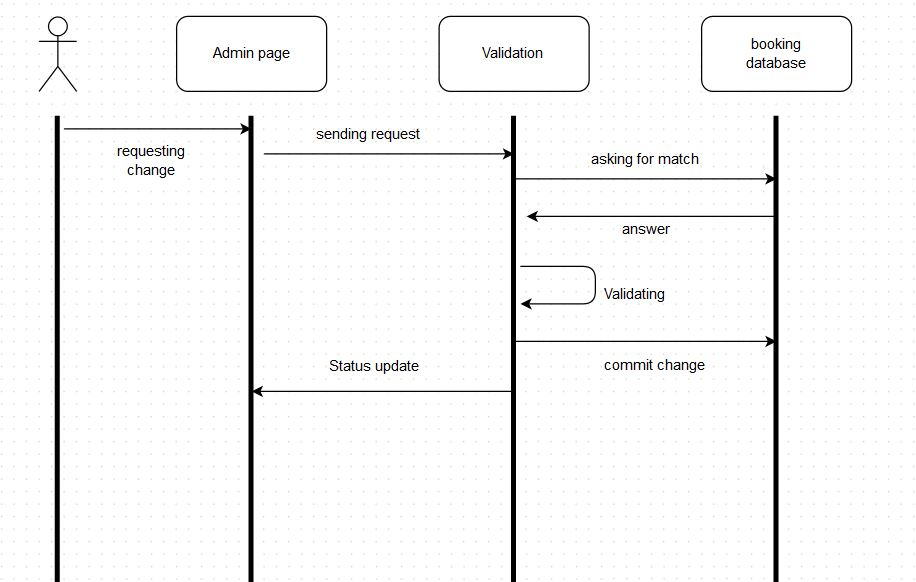
\includegraphics[scale=0.4]{adminInteraction.jpg}
\caption{Admin Interaction}
\end{figure}


\begin{figure}[H]
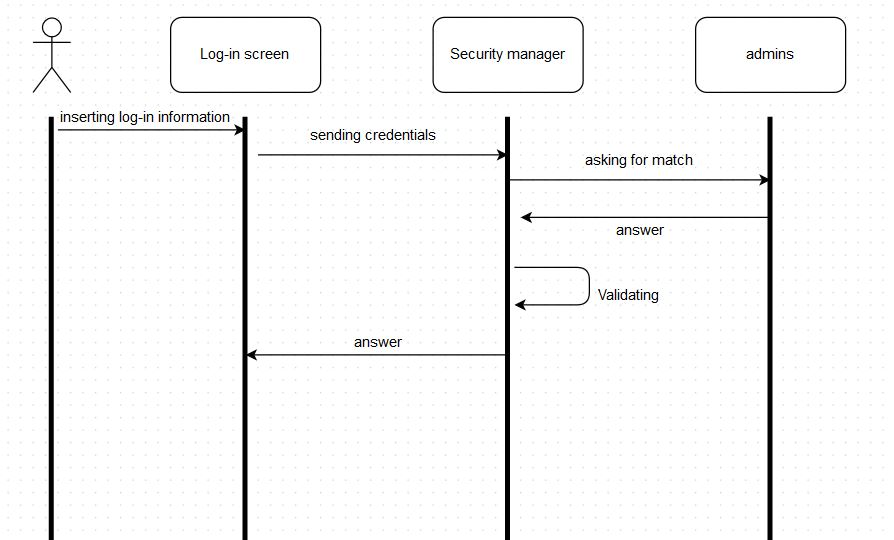
\includegraphics[scale=0.4]{adminLog-in.jpg}
\caption{Admin log-in}
\end{figure}


\begin{figure}[H]
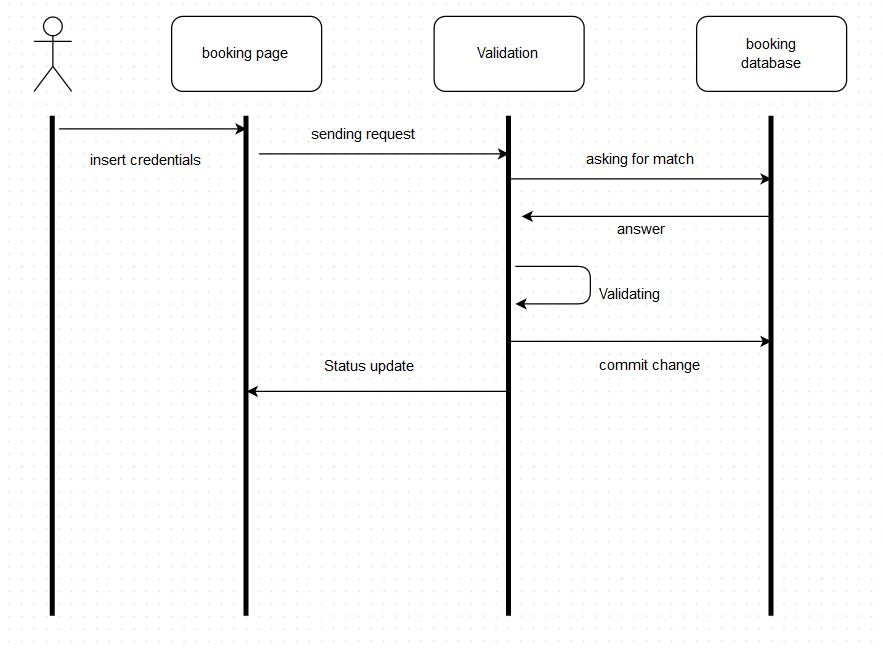
\includegraphics[scale=0.4]{customerLog-in.jpg}
\caption{Customer log-in}
\end{figure}
\newpage
\section{Systemdesign sammenfatning}
\textbf{Systemet som det er nu:}
Vi har foreløbigt lavet skabelonen til hjemmesiden, som den endeligt skal se ud. Dette er gjort i html og css kode. Derudover har vi implementeret links, så man kan navigere mellem siderne. 

\textbf{De væsentligste mangler:}
En administrator side hvor man kan ændre billederne på siden. 
Derudover skal der også være et bookingsystem, som kunder kan oprette bookninger, og som administratoren via administrator siden kan oprette/slette bookninger og hente information om kunden. Desuden mangler der et betalingssystem på siden.
\newpage
\section{Program- og systemtest}
Da vi endnu ikke har fået vores system op at køre, mener vi ikke at det, vi har indtil nu, ville være værd at tage med. I forhold til vores hjemmeside kan vi kun teste den visuelt ved at se, om linksne fører til de korrekte sider, og det gør de.
\newpage
\section{Brugergrænseflade og interaktonsdesign}
Fra menu bjælken kan brugeren navigerer sig rundt på hele hjemmesiden. Menu bjælken vil være tilstede lige meget hvor brugeren befinder sig henne på siden.

Siderne er uafhængig, så de har ingen relation til hinanden.
\newpage
\section{projektsamarbejdet}
Internt i gruppen arbejder vi godt sammen. Vi syntes dog at vi begynder at få travlt, hvis vi gerne vil ende ud med et mere eller mindre færdigt produkt, og har derfor aftalt at mødes hver mandag og bruge min. seks timer sammen på projektet. Inden vi går hjem mandag uddeler vi arbejdsopgaver, og aftaler hvad vi skal have nået, inden vi mødes igen ugen efter. 

Vi har indtil videre haft tre møder med kunden. Møderne foregår over Skype, da kunden bor i Venezuela. På trods af at afstanden kan være upraktisk, er kunden fleksibel med dato for møder, da vi blot mødes over Skype.

Under møderne tager vi referat i form af stikord, og dokumenterer de aftalte ændringer i projektaftalen og projektplanen, i rapporten. 

Under første møde d. 19. februar 2015 fik vi lavet en projektaftale med kunden.
Under andet møde d. 10. marts 2015 snakkede vi detaljer ift. bookingsystemet.
Udner tredje møde d. 15. april 2015 snakkede vi om valg af betalingssystem, samt om hvilke dele af projektet kunden helst så os nedprioritere i tilfælde af tidspres.

Vi har endnu ikke en fast dato for næste møde, da kunden som sagt er fleksibel, og vi derfor kan kontakte hende, når vi har brug for at diskutere projektet.

Vi har indset, at vi generelt set skal prioritere projektet højere, og vil derfor lave en tidsplan med deadlines til os selv. Første step bliver at lave en så deltaljeret som muligt projektplan.
Vi er motiverede af og glæder os til at gå igang med at kode, og lære hvordan et sådant system er bygget op. 
\newpage
\section{Litteraturreview}
\subsection{Designing for usability}
Denne artikel beskriver tre design principper, som Gould og Lewis mener er vigtige, men selv om de måske virker indlysende, bliver de ofte forsømt af udviklerne af flere årsager. Udviklerne undervurderer eller misforstår simpelthen nogle gange disse ”simple” principper. De tre principper: 

Fokus på målgruppe og opgaver. 
Hvor designeren må vide hvem målgruppen er og være i direkte kontakt med udviklerne, for at de kan analysere og studere målgruppens adfærd i stedet for at bare læse eller høre om dem. 

Simulation og prototype.
Målgruppen skal afprøve prototypen, hvor deres reaktion og ydeevne på systemet analyseres og observeres.

Test og omstrukturer.
Det sidste princip dækker over test af systemet og de fejl, som bliver fundet, skal rettes, og hvis det bliver nødvendigt, skal programmet omstruktureres og testes forfra.

Derefter uddyber de principperne, og forklarer, hvordan de kan anvendes i starten af design fasen efterfulgt af en test fase. De slutter deres diskussion ved at præsentere et case studie, hvor de anvender disse principper i et lyd besked system fra IBM.   

Det er svært at argumentere mod vigtigheden af disse principper, som måske virker meget basale, men det kan være meget let undervurdere vigtigheden af disse principper. Object-Oriented Software Engineering Using UML, Patterns, and Java bogen beskriver seks faser, når man udvikler et system.

Krav
Analyse
System Design
Objekt Design
Implementation
Test

Hvor den ligger meget vægt på samarbejde med kunden i form af modeller og grafiske illustration i stedet for at arbejde sammen med målgruppen, som jeg syntes artiklen ligger op til.

I vores projekt hvor vi har til opgave at designe og lave et online sommerhus booking system, forsøger vi at holde en løbende dialog med vores kunde. Vi fik først og fremmest nogle krav fra kunden, som vi skal overholde, men da de fleste var kommet på plads, og vi havde en nogenlunde idé om, hvad vi egentlig skulle lave i vores projekt. Dernæst har vi planer om at lave vores prototype af hjemmeside færdig, og derefter have et interview med vores kunde, for at se om de er tilfredse, eller om de har nogle ændringer. Efter det har vi planer om at nå ud til målgruppen med prototypen og høre deres mening om systemet, og om det er brugervenligt.
\subsection{A rational design process}
A Rational Design Process forklarer om hvad den rationelle design process er, og hvorfor det er så svært at lave en rationel struktur på sit projekt.

Kort sagt går et rationelt design ud på, at man stiller nogle helt præcise krav op for sit projekt. At man opdeler projektet i mindre og mindre detaljerede dele, indtil man har en fuldstændig plan for, hvordan man vil udføre sit projekt. Og at man dokumenterer alle beslutninger og ændringer, man foretager sig løbende.

Det er dog sjældent, at programmørens valg i den initielle designfase er særligt rationelle. Dette er der flere årsager til. Som vi selv har kunne mærke i vores projekt, vil der i starten ofte være uklarhed omkring, præcis hvad systemet skal kunne. Mange detaljer dukker altid op løbende under design- og programmeringsprocessen, og det er derfor ikke muligt fra start af at lave en nøjagtig plan. Selv hvis det var muligt at kende til alle projektets detaljer på en gang, vil det simpelthen være for stor en mundfuld information, til at det er muligt for den menneskelige hjerne at lave et endeligt softwaredesign. Der sker ofte ændringer i, hvad systemet skal indebære. Disse ændringer har ofte betydning for designet, og man ville altså alligevel ende med et andet design end det første “rationelle design” man havde konstrueret. Endeligt sker det tit, at man skal viderearbejde allerede eksisterende software, som allerede har et design. Et rationelt design kan også udelukke muligheden for nye og anderledes ideer til design, inspireret af andre projekter, hvis design ikke nødvendigvis er særligt rationelt, men som på en anden måde virker optimalt for ens projekt.

På trods af alle disse stopklodser for en rationel design process er der også mange positive sider ved at forsøge at lave et rationelt design. Der researches derfor en del i en struktureret ”opskrift” på software design.
Ligger man tid og kræfter i at få lavet et godt solidt design, før man går i gang med at kode, bliver man tvunget til at reflektere over hele projektet, og tage stilling til hvilke udfordringer man måske støder på. Dette vil spare én tid i den anden ende.

Vi er opsatte på at forsøge os med at lave en detaljeret projektplan, da vi efterhånden begynder at forstå nødvendigheden af at have et godt overblik over det system, vi arbejder på. Vi vil også få lavet noget ordentlig dokumentation, for de valg vi tager, så vi på senere tidspunkter kan finde svar på, hvorfor vi valgte at gøre som vi gjorde. 
Dog er der mange ting, vi har svært ved at forestille os på dette tidlige stadie, især fordi at ingen af os har nogen programmeringserfaring. Det gør det f.eks. svært for os at vide, hvordan vi egentlig skal inddele projektet i moduler/subsystems, samt hvor lang tid hver del af projektet vil tage.

Vi anser opskriften på hvordan man laver et rationelt design som en slags guide og inspiration til, hvordan man kan gribe et projekt an. I forsøget på at følge opskriften på det rationelle design vil man eksempelvis lægge et større arbejde i at finde de små detaljer og risici ved projektet så tidligt som muligt og dermed undgå for meget back-tracking.
Ved efterfølgende at skrive sin dokumentation og projektplan som hvis man havde fulgt det perfekte design, altså ”fake” den ideelle process, bliver man stadig tvunget til at være mere reflekteret og forberedt, og gør dermed projektet og ens egen arbejde mere struktureret. 
\end{document}